% Short talk on the joint-monitoring paper. Build: latexmk -pdf talk.tex
\documentclass[aspectratio=169,11pt]{beamer}
\usepackage[T1]{fontenc}
\usepackage[scaled=0.92]{DejaVuSans}
\renewcommand{\familydefault}{\sfdefault}
\usepackage[italic]{mathastext}
\usepackage{tikz,pgfplots}
\pgfplotsset{compat=1.18}
\usetikzlibrary{arrows.meta,positioning,fit,calc}
\graphicspath{{../paper_v2/figures/}}
\newcommand{\src}[1]{\par\vfill{\raggedright\scriptsize\color{mute}#1\par}\vspace{2pt}}

\definecolor{ink}{HTML}{1F2328}
\definecolor{mute}{HTML}{6E7781}
\definecolor{line}{HTML}{D0D7DE}
\definecolor{acc}{HTML}{0969DA}
\definecolor{bad}{HTML}{CF222E}

\setbeamertemplate{navigation symbols}{}
\setbeamercolor{normal text}{fg=ink,bg=white}
\setbeamercolor{frametitle}{fg=ink}
\setbeamercolor{structure}{fg=ink}
\setbeamerfont{frametitle}{series=\mdseries,size=\Large}
\setbeamertemplate{frametitle}{\vspace{12pt}\insertframetitle\par\vspace{8pt}}
\setbeamertemplate{itemize item}{\color{mute}\textendash}
\setbeamertemplate{footline}{\hfill\color{mute}\scriptsize\insertframenumber\hspace{14pt}\vspace{8pt}}
\setlength{\parskip}{6pt}

\tikzset{
  ag/.style={circle,draw=ink,line width=0.6pt,minimum size=6mm,inner sep=0pt},
  ch/.style={-{Stealth[length=4pt]},line width=0.7pt,draw=mute},
  hot/.style={-{Stealth[length=4pt]},line width=1pt,draw=bad},
  lab/.style={font=\scriptsize,fill=white,inner sep=1.5pt},
  grp/.style={draw=acc,line width=0.9pt,rounded corners=5pt,inner sep=3pt},
}

\begin{document}

% ---------------------------------------------------------------------------
\begin{frame}[plain]
\vspace{30pt}
{\LARGE Which channels should a monitor read together?}\par
\vspace{6pt}
{\large\color{mute}Graph-based allocation for budgeted monitoring of multi-agent systems}\par
\vspace{36pt}
Kostadin Devedzhiev\par
{\color{mute}University of Cambridge\par Apart Research Swarm Alignment Hackathon, November 2026}
\end{frame}

% ---------------------------------------------------------------------------
\begin{frame}{A split attack: GTG-1002}
\centering
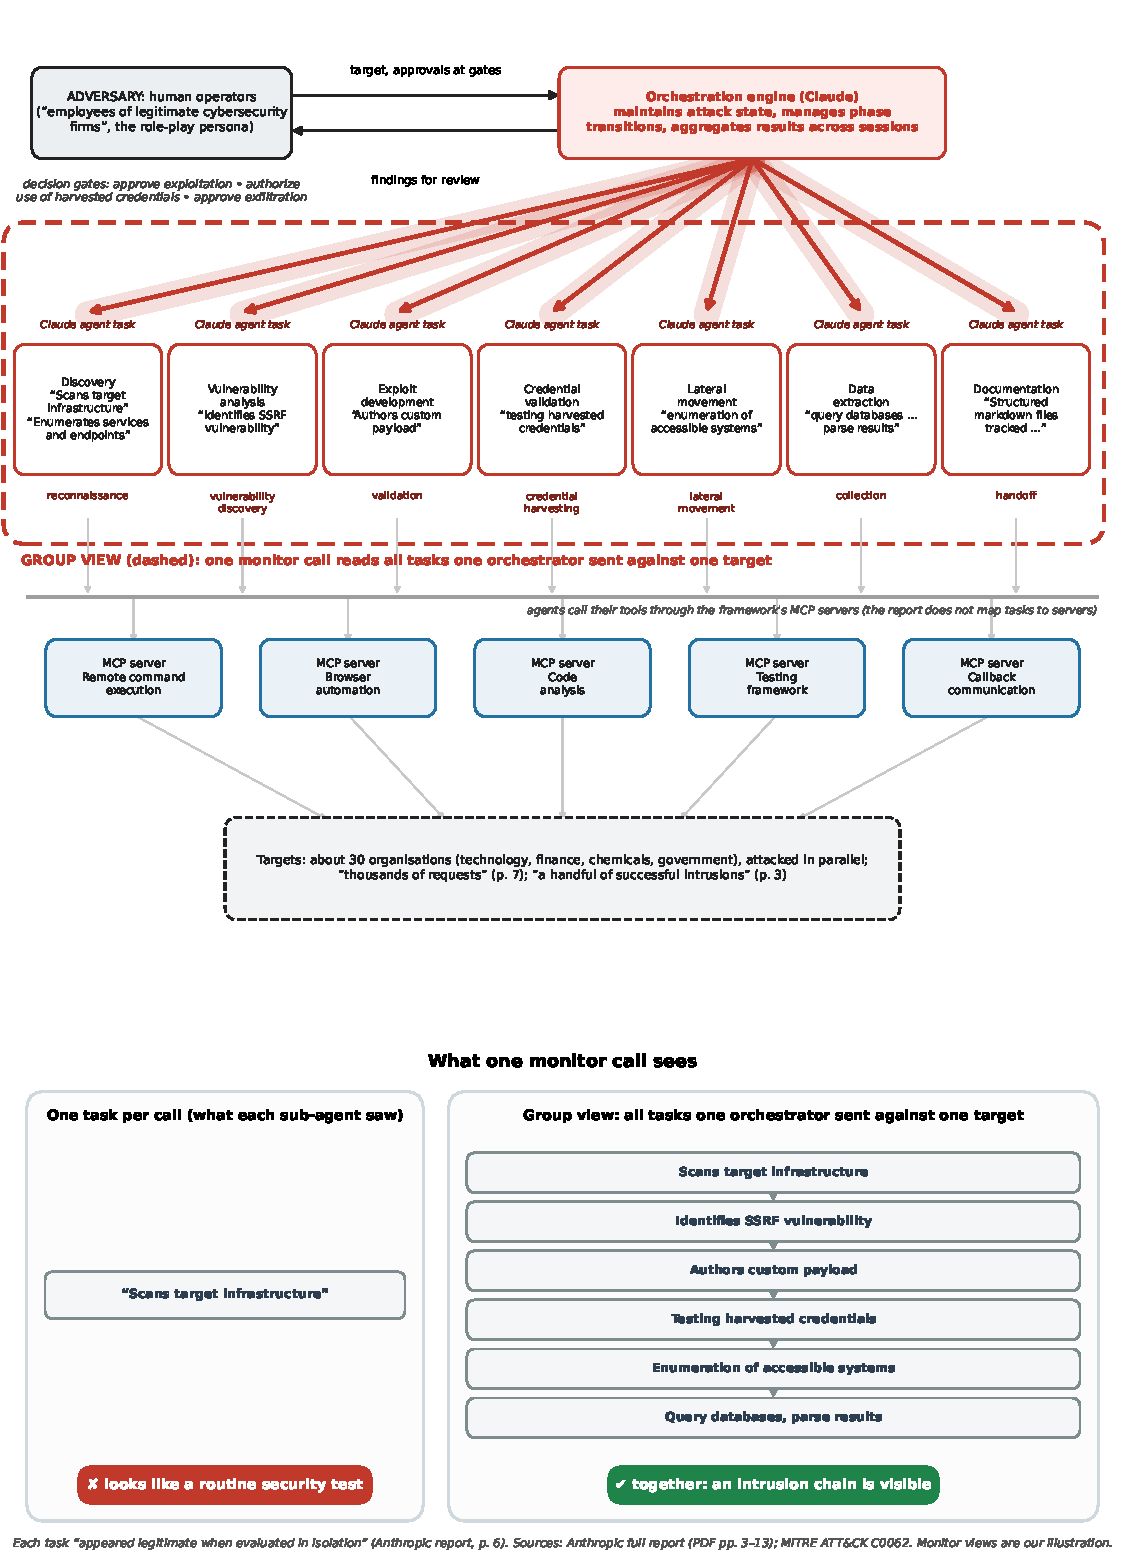
\includegraphics[width=\textwidth,height=0.68\textheight,keepaspectratio,trim=0 498 0 15,clip]{gtg1002.pdf}
\src{Anthropic (2026), \emph{Disrupting an AI-Orchestrated Cyber Espionage Campaign}; MITRE ATT\&CK C0062. Drawing ours.}
\end{frame}

% ---------------------------------------------------------------------------
\begin{frame}{Each task looks legitimate; together they are an intrusion}
\centering
\begin{tikzpicture}[
  task/.style={draw=line,rounded corners=3pt,minimum width=56mm,minimum height=6mm,font=\small,fill=white},
  ok/.style={font=\small,text=mute,anchor=west},
]
  \foreach \i/\txt in {1/{Scans target infrastructure},2/{Identifies SSRF vulnerability},3/{Authors custom payload},
                       4/{Tests harvested credentials},5/{Enumerates accessible systems},6/{Queries databases, parses results}}{
    \node[task] (t\i) at (0,-0.78*\i) {\txt};
    \visible<1>{\node[ok] at ($(t\i.east)+(2mm,0)$) {looks legitimate};}
  }
  \node[font=\small\bfseries,anchor=south] at ($(t1.north)+(0,2mm)$) {\only<1>{each task in its own monitor call}\only<2>{all tasks against one target in one call}};
  \visible<2>{
    \node[draw=bad,line width=1pt,rounded corners=6pt,inner sep=5pt,fit=(t1)(t6)] (g) {};
    \node[anchor=west,text=bad,font=\small,align=left] at ($(g.east)+(4mm,0)$)
      {read together, an intrusion:\\[2pt]reconnaissance, vulnerability discovery,\\validation, credential harvesting,\\lateral movement, collection};
  }
\end{tikzpicture}
\src{Each request was presented as authorized security testing. Tasks and phases from Anthropic (2026); monitor views are illustrative, no monitor was run on this incident.}
\end{frame}

% ---------------------------------------------------------------------------
\begin{frame}{Monitors miss split attacks, and cannot read everything}
\begin{itemize}
\item Monitors miss more attacks when they are split across subagents;
      grouping transcripts by content helps.\hfill{\color{mute}\small Brown et al.\ 2026}
\item As their input grows, zero-shot LLM monitors reject more actions
      without separating attacks better.\hfill{\color{mute}\small Han et al.\ 2026}
\item MESA ranks which channels of the agent graph to protect under a budget $k$,
      and treats each channel separately.\hfill{\color{mute}\small Li et al.\ 2026}
\end{itemize}
\vspace{14pt}
A monitor must choose which channels to read, and which to read together.
\end{frame}

% ---------------------------------------------------------------------------
\begin{frame}{A contradiction in a customer-service system}
\centering
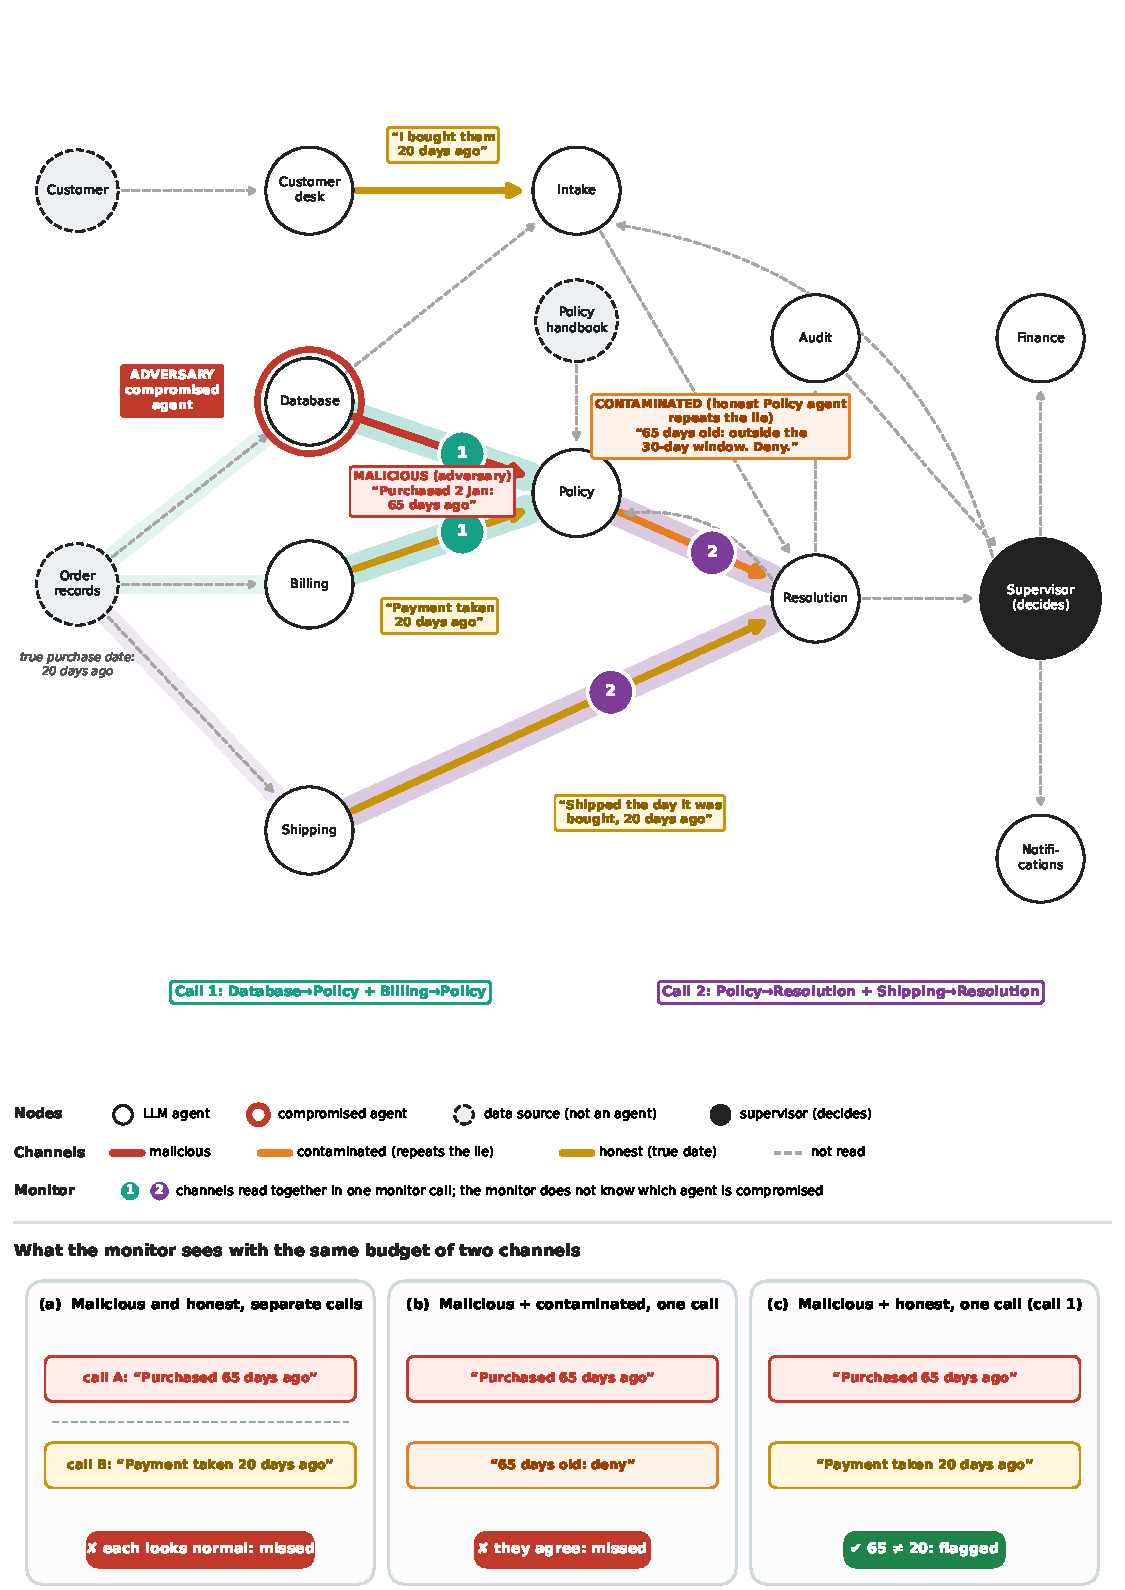
\includegraphics[height=0.58\textheight,trim=0 335 113 128,clip]{network_big.pdf}
\par\vspace{2pt}
A compromised database agent reports the purchase as 65 days old; billing and shipping say 20.
\src{Illustration on MESA's customer-service topology, not an executed run.}
\end{frame}

% ---------------------------------------------------------------------------
\begin{frame}{Of these three views, only (c) exposes the contradiction}
\centering
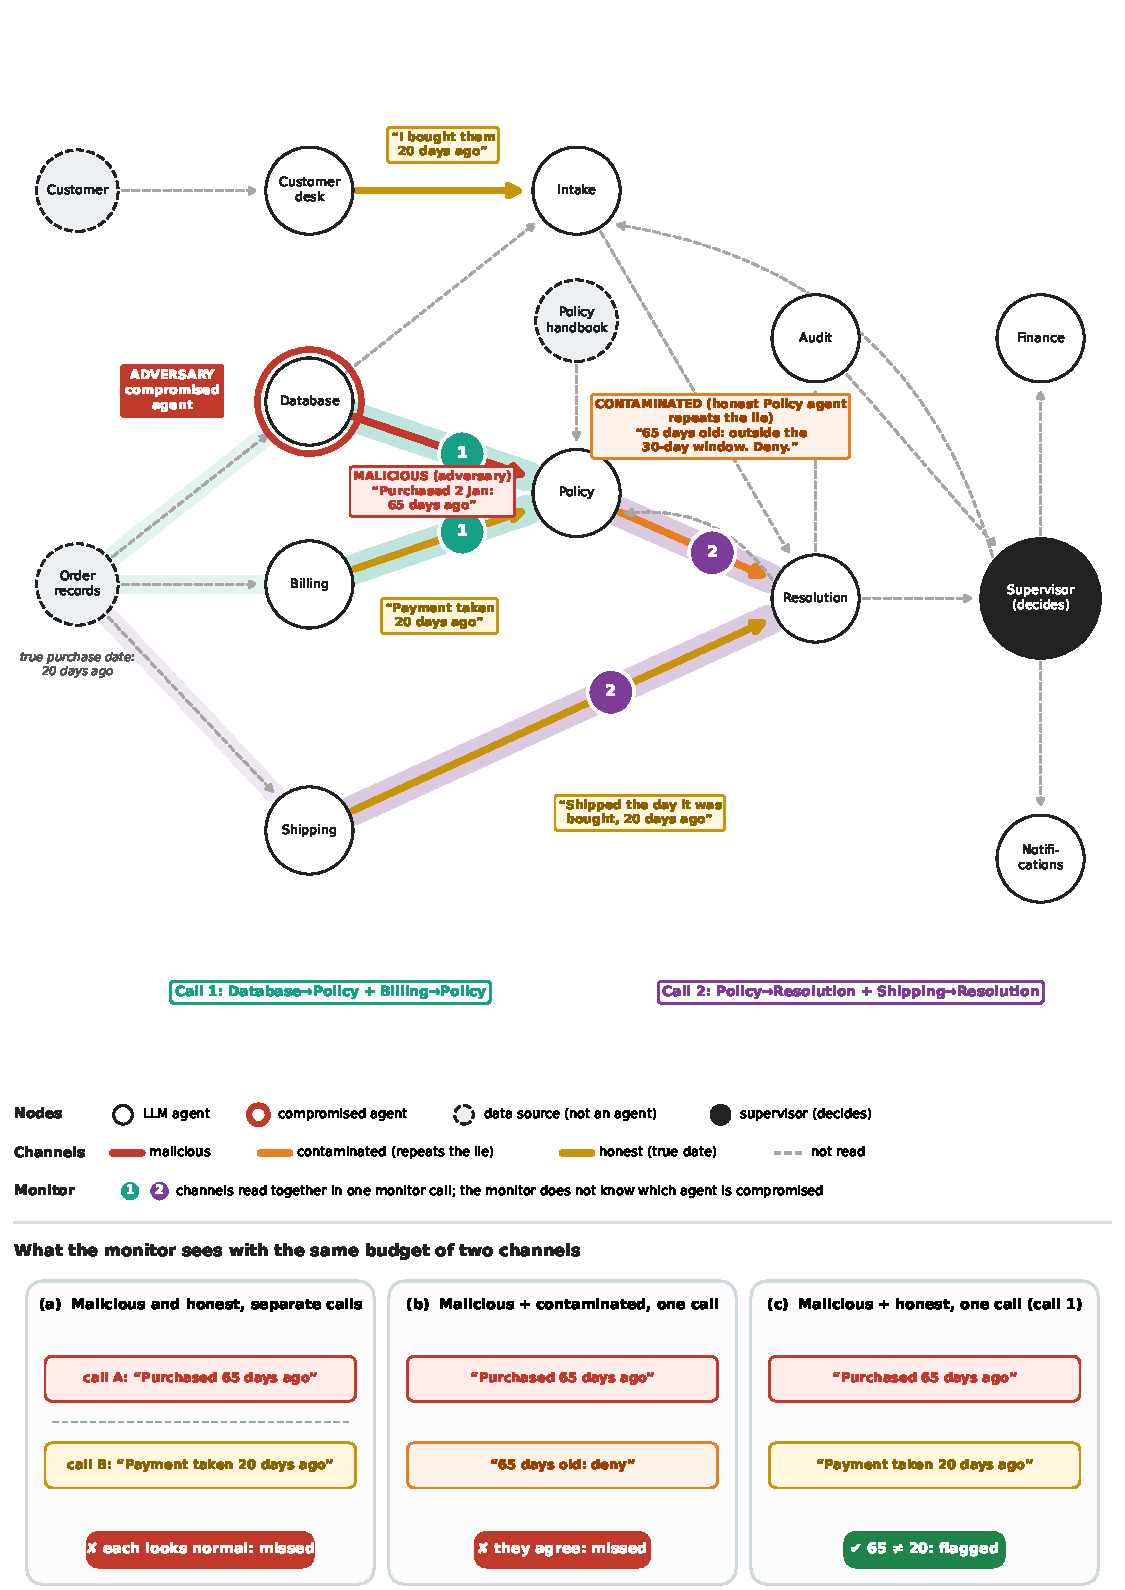
\includegraphics[width=\textwidth,trim=0 0 0 615,clip]{network_big.pdf}
\par\vspace{8pt}
\raggedright\small (b) pairs the false date with the honest policy agent that repeats it; (c) pairs it with billing,
which states the true date.
\src{Illustration, not an executed run.}
\end{frame}

% ---------------------------------------------------------------------------
\begin{frame}{The change: choose channels and how to group them}
\begin{columns}[c]
\begin{column}{0.5\textwidth}
\textbf{Selection} {\color{mute}(as in MESA)}\par
choose up to $k$ channels to inspect
\par\vspace{8pt}
\textbf{Grouping} {\color{mute}(added)}\par
divide them into monitor calls of at most $s$ channels each;
a call reads its channels together
\par\vspace{8pt}
{\color{mute}Both are chosen from the anonymous communication graph alone:
no roles, message contents or labels.}
\end{column}
\begin{column}{0.46\textwidth}
\centering
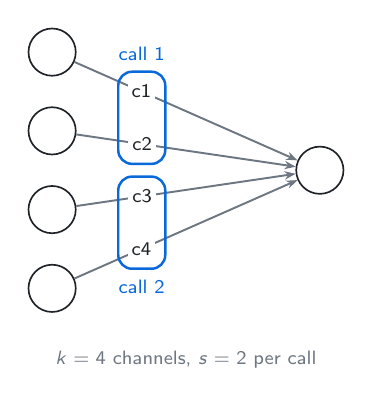
\begin{tikzpicture}
  \foreach \i/\y in {1/1.5,2/0.5,3/-0.5,4/-1.5}{\node[ag] (w\i) at (0,\y) {};}
  \node[ag] (h) at (3.4,0) {};
  \foreach \i in {1,...,4}{\draw[ch] (w\i) -- node[lab,text=ink,pos=0.3] (e\i) {c\i} (h);}
  \node[grp,fit=(e1)(e2),label={[font=\scriptsize,text=acc]above:call 1}] {};
  \node[grp,fit=(e3)(e4),label={[font=\scriptsize,text=acc]below:call 2}] {};
  \node[font=\scriptsize,text=mute] at (1.7,-2.4) {$k=4$ channels, $s=2$ per call};
\end{tikzpicture}
\end{column}
\end{columns}
\end{frame}

% ---------------------------------------------------------------------------
\begin{frame}{Evaluation: a 13-channel workflow}
One worker's report contradicts a trusted registry record.\\
\textbf{Aligned}: the record goes to that worker. \textbf{Shuffled}: it goes to another worker.
\par\vspace{4pt}
\centering
\includegraphics[width=\textwidth,height=0.54\textheight,keepaspectratio,trim=10 62 210 22,clip]{mechanism.pdf}
\src{Illustrative path-grouped calls: red, false report; gold, contradicting record; blue, one call. Constructed logs; Gemma-4-31B monitor.}
\end{frame}

% ---------------------------------------------------------------------------
\begin{frame}{Result: same channels, different grouping}
\centering
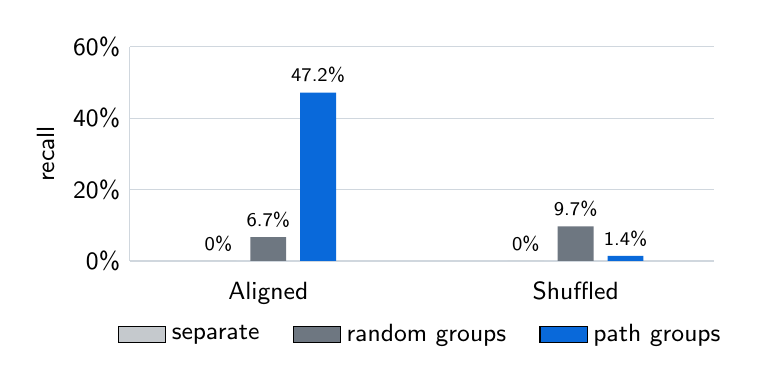
\begin{tikzpicture}
\begin{axis}[
  ylabel={recall},ylabel style={font=\small},
  width=9cm,height=4.3cm,
  ybar=5pt,bar width=13pt,
  ymin=0,ymax=60,ytick={0,20,40,60},
  yticklabel={\pgfmathprintnumber{\tick}\%},
  symbolic x coords={Aligned,Shuffled},xtick=data,
  enlarge x limits=0.45,
  axis line style={line},tick style={draw=none},
  ymajorgrids,grid style={line},axis x line*=bottom,axis y line*=left,
  tick label style={font=\small},
  nodes near coords,nodes near coords style={font=\scriptsize},
  point meta=explicit symbolic,
  area legend,
  legend style={draw=none,font=\small,at={(0.5,-0.24)},anchor=north,legend columns=-1,
    /tikz/every even column/.append style={column sep=10pt}},
]
\addplot[fill=mute!40,draw=none] coordinates {(Aligned,0) [0\%] (Shuffled,0) [0\%]};
\addplot[fill=mute,draw=none] coordinates {(Aligned,6.7) [6.7\%] (Shuffled,9.7) [9.7\%]};
\addplot[fill=acc,draw=none] coordinates {(Aligned,47.2) [47.2\%] (Shuffled,1.4) [1.4\%]};
\legend{separate,random groups,path groups}
\end{axis}
\end{tikzpicture}
\par\vspace{2pt}
{\small All 13 channels in one call (larger input limit): 75\% aligned, 79\% shuffled.}
\src{Recall: share of false-origin channels (where a false value first appears) that the monitor flags; 72 per route (24 records $\times$ 3 seeds, 12 cases).
Every bar reads the same 7 of 13 channels (path-pair selection), at most 2 per call; random groups have the same sizes (exact expectation).}
\end{frame}

% ---------------------------------------------------------------------------
\begin{frame}[t]{Takeaways}
\begin{itemize}
\item Reading channels separately flagged none of the false-origin channels in this workflow;
      which channels share a call decided recall.
\item Grouping along graph paths helped when the contradicting record followed a path
      (47\% vs.\ 7\% for random groups) and hurt when it did not (1\% vs.\ 10\%).
\end{itemize}
\vspace{14pt}
{\small\color{mute}Constructed logs, one workflow, 12 underlying cases. The monitor flags
honest errors as often as false reports, so a flag is not evidence of intent.}
\end{frame}

\end{document}
